\documentclass[12pt]{article}
\usepackage{fullpage,url,amssymb,epsfig,color,xspace,tikz,amsmath, amsthm}
\usetikzlibrary{calc,shapes.multipart,chains,arrows}
\usepackage{graphicx}
\begin{document}

\begin{center}
    \textbf{\huge Tutorial 4}
\end{center}


\section{Stack}
\begin{itemize}
    \item A stack is an ordered container of data that enforces a LIFO policy on adds/removes
    \item Permitted operations: push, pop, peek, isEmpty
    \item e.g. back and forward putton on a browser. Any idea how to implement this?
\end{itemize}

\begin{center}
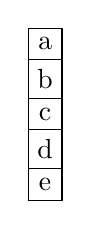
\begin{tikzpicture}[stack/.style={rectangle split, rectangle split parts=#1,draw, anchor=center}]
    \node[stack=5]  {
        \nodepart{one}a
        \nodepart{two}b
        \nodepart{three}c
        \nodepart{four}d
        \nodepart{five}e
    };
\end{tikzpicture}
\end{center}

\section{References}
\begin{itemize}
    \item References are like pointers
    \item The reference parameter is just another name (i.e., an alias) for the
    variable in the calling context
\end{itemize}
\textbf{Q:} Is the valid?
\begin{verbatim}
int foo(int &i) {return i;}
int main() {foo(1);}
\end{verbatim}

\section{Exercises}
\begin{enumerate}
    \item Write a recursive function \textbf{bool isCircular(const List \&l)} that returns true if a singly linked list 
    is circular and false otherwise. You may use helper functions if you wish.
    \item Write a recursive function \textbf{int findMin(const List \&l)} that returns the minimum value stored in a 
    singly linked list of integers. You may use helper functions if you wish.
    \item Write a recursive function int recursivePower(int base, int exponent) that returns baseexponent. 
    For example, \textbf{recursivePower(4, 2)} should return 16. You should not need to use helper functions. 
    Try to solve it in $O(\log n)$ time. (Hint: $x^{10} = x^5 \times x^5$)
\end{enumerate}
\end{document}  